\section{Efficient subclasses of graphs}
In this section a case when the input graph (regular language or finite automata, respectively) is fixed and context-free grammar is arbitrary, will be considered.
\subsection{Directed acyclic graphs and trees}
The most trivial example of ``easy'' for our circuit graphs are directed acyclic graphs. It is not difficult to see that all words accepted by an appropriate finite automata have length no more than $O(n)$, where $n$ is number of nodes in graph. So, we obtain the following.
\begin{corollary} 
Let  $G = (\Sigma, N, P)$ be a context-free grammar and $D=(V, E, \Sigma)$ be a directed acyclic labelled graph with $n$ nodes. Then CFL-reachability problem for $G$ and $D$ is in $NC^2$.
\end{corollary}
\subsection{Partially ordered automata}

Partially ordered automata generalize the previous case. \textit{Partially ordered automata} are finite automata where the transition relation has a partial
order on states. It means that as soon as a state is left during the run, it is never visited again.  As a consequence, all cycles of partially ordered automata are only self-loops.


Notice that the lengths of accepted words are not bounded in this case because of existence of self-loops. We will show that the value of $\mathzapf{L}$ still stays polynomial despite infinite lengths of accepted words.
\begin{lemma}
\label{partord}
Let  $G = (\Sigma, N, P)$ be a context-free grammar in Chomsky normal form and $\mathzapf{A}$ be a partially ordered automaton with $n$ states. Then the length of the maximum in all nonterminals and all pairs of states shortest path labelled by a string from $L(G)$ ($\mathzapf{L}$) is no more than $O(n)$.
\end{lemma}
\begin{proof} \textit{(Sketch)}.
Assume that there is loop on some vertex $i$. Consider the maximum possible length of path $i\pi i$ from $i$ to $i$. There two cases of parse subtrees for $l(i\pi i)$. First case is when $l(i\pi i)$ has a distinct parse subtree. Then, the height of such tree is no more than $|N|$, because there are only $|N|$ unique triples in form of $(A, i, i)$, where $A \in N$. The maximum number of leaves in a parse tree of height $h$ (if the grammar is in Chomsky normal form) is $2^h=2^{|N|}$.
\\The second case is when the $l(i\pi i)$ doesn't have a distinct parse tree. It means that there is no derivation $A \stackrel {*}{\Rightarrow } l(i\pi i)$ for $A \in N$. Let $T$ be the smallest parse tree which yields a string $l(i \pi_1 k)$, where $l(i\pi i)$ is substring of $l(i \pi_1 k)$. Because the grammar is in the Chomsky normal form, derivation tree for $l(i \pi k)$ looks as illustrated in Figure \ref{partordtree}. The maximum length of $l(i\pi i)$ is equal to the maximum height of a parse tree for string $l(i \pi_1 k)$. It is equal to number of unique triples $(A, i, k):|N|$. Case for $l(m \pi_1 i)$ is hold symmetrically. Finally we have the $\mathzapf{L}$ in $O(2^{|N|}n) + O(n) = O(n)$ in the worst case (there are loops on every vertex).
\end{proof}


Applying Lemma \ref{partord} and Corollary \ref{coldepth}, we have the following corollary.
\begin{corollary} 
Let  $G = (\Sigma, N, P)$ be a context-free in Chomsky normal form and $\mathzapf{A}$ be a partially ordered automaton with $n$ states. Then CFL-reachability problem for $G$ and $\mathzapf{A}$ is in $NC^2$.
\end{corollary}
\begin{figure}
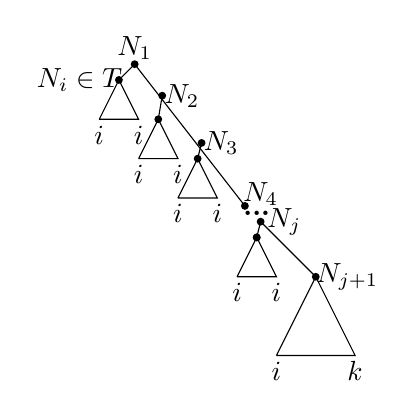
\begin{tikzpicture}
\draw(2.5, 0) -- (3.5,0) -- (3, 1) -- (2.5, 0);
\draw(2, 1) -- (2.5,1) -- (2.25, 1.5) --(2, 1);
\draw(1.25, 2) -- (1.75,2) -- (1.5, 2.5) --(1.25, 2);
\draw(0.75, 2.5) -- (1.25,2.5) -- (1, 3) --(0.75, 2.5);
\draw(0.25, 3) -- (0.75,3) -- (0.5, 3.5) --(0.25, 3);
\draw(3,1) -- (2.3,1.7);
\draw(2.25, 1.5) -- (2.3,1.7);
\draw(2.1, 1.9) -- (0.7, 3.7);

\draw(1.5, 2.5) -- (1.55,2.7);
\draw(1,3) -- (1.05,3.3);
\draw(0.5, 3.5) -- (0.7, 3.7);

\node (start) at (0, 0) {}; 
\node (s) at (2.25 , 1.8) {\textbf{...}}; 
\node (q) at (2.5 , -0.2) {$i$}; 
\node (q2) at (3.5 , -0.2) {$k$}; 
\node (q3) at (2, 0.8) {$i$}; 
\node (q4) at  (2.5,0.8) {$i$}; 
\node (q5) at  (1.25, 1.8) {$i$}; 
\node (q6) at  (1.75,1.8)  {$i$}; 
\node (q7) at  (0.75, 2.3) {$i$}; 
\node (q8) at  (1.25,2.3)  {$i$}; 
\node (q9) at  (0.25, 2.8) {$i$}; 
\node (q10) at  (0.75,2.8)  {$i$}; 

\node (q11) at  (3.4, 1)  {$N_{j+1}$}; 
\node (q11) at  (0.7, 3.9)  {$N_1$}; 
\node (q11) at  (1.3,3.3)  {$N_2$}; 
\node (q11) at  (1.8, 2.7)  {$N_3$}; 
\node (q11) at  (2.6,1.7)  {$N_j$}; 
\node (q11) at  (0, 3.5)  {$N_i \in T$}; 
\node (q11) at  (2.3, 2.05)  {$N_4$}; 


\node [circle, fill=black, inner sep = 1pt, minimum size=0.5pt] at (3, 1) {};
\node [circle, fill=black, inner sep = 1pt, minimum size=0.5pt] at  (2.25, 1.5)  {};
\node [circle, fill=black, inner sep = 1pt, minimum size=0.5pt] at (2.3,1.7) {};
\node [circle, fill=black, inner sep = 1pt, minimum size=0.5pt] at (0.7, 3.7) {};
\node [circle, fill=black, inner sep = 1pt, minimum size=0.5pt] at  (1.55,2.7) {};
\node [circle, fill=black, inner sep = 1pt, minimum size=0.5pt] at  (1.05,3.3) {};
\node [circle, fill=black, inner sep = 1pt, minimum size=0.5pt] at (2.25, 1.5) {};
\node [circle, fill=black, inner sep = 1pt, minimum size=0.5pt] at  (1.5, 2.5) {};
\node [circle, fill=black, inner sep = 1pt, minimum size=0.5pt] at  (1, 3) {};
\node [circle, fill=black, inner sep = 1pt, minimum size=0.5pt] at  (0.5, 3.5) {};
\node [circle, fill=black, inner sep = 1pt, minimum size=0.5pt] at  (2.1, 1.9) {};
\end{tikzpicture}
\\
	\caption{A derivation tree for $l(i \pi k)$, $T \in N$ is the set of terminals.}
\label{partordtree}
\end{figure}


Famous examples of language accepted by partially ordered automata are \textit{piecewise testable languages} \cite*{simon1972hierarchies, masopust2019partially}. A regular language over an alphabet $\Sigma$ is \textit{piecewise testable} if it is a finite Boolean combination of languages of the form $\Sigma^*a_1\Sigma^*a_2\Sigma^* ... \Sigma^*a_k$, where $a_1, a_2, ... , a_k \in \Sigma$, $k \ge 0$. 